\documentclass[12pt,t]{beamer}
\usetheme[greyauthor, % Grå tekst forfatter som KU vil have
         unit=NAT, % Ændre til NAT, KU, eller unit=ics (diku)
         dk, % Sprog
         %style=simple, % Vandmærke eller billede
         footstyle=low, % Fjern stor footer
         wmark, % vandmærke på hver side
         logoplace=left % Logo til venstre
         %,sidebar % makes sidebar
         ]{Frederiksberg}
% nat for Science, ku for generic or unit=ics for DIKU
% Tilføj style=simple for vandmærke
\usepackage{listings} % Pakke til kode
\usepackage{pslatex}        % pæn skrift
\usepackage[utf8]{inputenc} % Implementerer Unicode
\usepackage{algpseudocode}
\usepackage{algorithm}

\title{Studiepraktik 2016}
\subtitle{Algoritmer og problemløsning}
\author{
        Arinbjörn Brandsson \\
        Benjamin Rotendahl  \\
        Mathias Fleig Mortensen \\
        Christopher Mulvad Groot\\
}

\date[]{\today}


\begin{document}

\frame[plain]{\titlepage}
 \frame{\tableofcontents}

\section{Dagens program}

\begin{frame}
    \frametitle{Program for idag}
    \begin{block}{Indtil kl 11.45}
        \begin{itemize}
            \item Algoritme design og metoder. \pause
            \item Hvordan man kan sammenligne forskellige løsninger. \pause
            \item Hvad er grænserne for algoritmer? \pause \alert{Historie tid!}
        \end{itemize}
    \end{block}
    \pause
    \begin{block}{Fra 13 til 14.30}
        \begin{itemize}
            \item Øvelser i algoritmer \pause
            \item Sjove gåder \pause
            \item Opsamling og spørgsmål
        \end{itemize}
    \end{block}
\end{frame}


\section{Introduktion til algoritmer}
    \begin{frame}[c]{Hvad er en Algoritme?}
        \begin{quote}
            An algorithm is a self-contained step-by-step set of operations to
            be performed that can be expressed within a finite amount of space
            and time and in a well-defined formal language.
        \end{quote}
        \pause
        \begin{block}{På dansk}
            En algoritme er en \alert{opskrift} på hvordan et bestemt problem
            kan løses.
        \end{block}
    \end{frame}


    \begin{frame}[plain]{Havregryns algoritme}
        \begin{block}{Eksempel}
        \vspace{-1.5em}
        \begin{algorithm}[H]
            \caption{\newline Indgangsbetingelser: En skål, mælk, havregryn
                     \newline Udgangsbetingelser: Morgenmad
            }
            \begin{algorithmic}
                \While{Skålen ikke er fyldt}
                    \State Hæld Gryn i Skålen
                \EndWhile
                \If{Jeg er tyk}
                    \State mælk = Minimælk
                \Else
                    \State mælk = Letmælk
                \EndIf
                \While{Skålen ikke er fyldt}
                    \State Hæld mælk i Skålen
                \EndWhile
            \end{algorithmic}
        \end{algorithm}
        \end{block}
    \end{frame}

    \begin{frame}
        \frametitle{Krav til en algoritme?}
        \begin{block}{Krav til en algoritme}
        \begin{description}
            \item[Veldefineret] Ingen tvetydigheder og vendinger som:``
            så tager du det bedste resultat $\dots$'' \pause
            \item[Terminerer] Den må ikke køre for evigt, du skal garantere
            at den rent faktisk finder sit svar. \pause
            \item[input og output] Jeg skal vide at hvis jeg giver
            den $A$ så returnerer den $B$. \pause
            \item[Kan bevises] Det er muligt både at bevise korrekthed og
            køretid for algoritmen.
        \end{description}
        \end{block}
    \end{frame}

    \begin{frame}[t]{Eksempler på algoritmer}
        Algoritmer bruges inden for alle former for problemløsnings. \pause
        \begin{block}{Bioinformatik}
            \emph{Longest commen subsequence: } Sammenligning af DNA strenge
            for at se hvor beslægtet to strenge er. \pause
        \end{block}
        \begin{block}{Primtals faktorisering}
            Bruges i \emph{kryptering: } Basis for at vi kan have sikker
            kommunikation. \pause
        \end{block}

        \begin{block}{Machine Learning}
            En samling af algoritmer der selv kan lære og finde egenskaber
            i store data sæt. Gør det muligt at løse problemer der før var
            uden for menneskers kunnen.
        \end{block}
    \end{frame}


\section{Algoritme vs Algoritme}
    \begin{frame}[t]{Valget af algoritme}
        \begin{exampleblock}{Soterings algoritmer}
            Givet en liste af $n$ tal ønsker vi at returnere en sorteret liste
            af længde $n$.
        \end{exampleblock}
        \pause
        \vspace{-2em}
        \begin{columns}
            \begin{column}{0.5\textwidth}
                \begin{block}{Hold $A$}
                    \begin{itemize}
                        \onslide<+->{\item Har en computer}
                        \onslide<+->{\item Bruger algoritmen \emph{Merge Sort}}
                        \onslide<+->{\item De kan sortere $10$ millioner tal på
                                     under $20$ minutter}
                        \onslide<+->{\item De kan sortere $100$ millioner tal på
                                    $4$ timer.}
                    \end{itemize}
                \end{block}
            \end{column}
            \begin{column}{0.5\textwidth}
                \begin{block}{Hold $B$}
                    \begin{itemize}[<+->]
                    \item Har en computer der er $1000$ gange hurtigere end
                    hold A
                    \item Bruger algoritmen \emph{Insertion Sort}
                    \item De kan sortere $10$ millioner tal på $5$ timer.
                    \item De kan sortere $100$ millioner tal på \alert{23 dage!}
                    \end{itemize}
                \end{block}
            \end{column}
        \end{columns}
    \end{frame}

    \begin{frame}[t]{Sammenligning af Algoritmer}
        \begin{quote}
            Vi bruger begrebet \emph{Køretid} for at beskrive hvordan tiden en
            algoritme bruger stiger med input.
        \end{quote}
        \pause
        \vspace{-1em}
        \begin{block}{Definition på køretid}
            En øvregrænse for den tid der bliver brugt på at løse et problem af
            størelse $n$. Skrives som
            $$
                O(n), O(n^2), O(n \lg n), O(n!), O\left( \frac{a}{b} \right)
            $$
        \end{block}
        \pause
        \begin{exampleblock}{Algoritme for minimums funktionen}
            Givet en liste $X = [x_1,x_2,\dots,x_n]$ ønsker vi at returnere det
            mindste tal i listen. Hvad er algoritmen og hvad er køretiden?
        \end{exampleblock}
    \end{frame}

    \begin{frame}{Minimums algoritme}
        \begin{block}{Eksempel}
        \vspace{-1.5em}
        \begin{algorithm}[H]
            \caption{\newline Input: En liste $X=[x_1,x_2, \dots, x_n]$
                     \newline Ouput: Det mindste tal i listen.
            }
            \begin{algorithmic}
                \State min = $x_1$
                \For{$x_i$ in X}
                    \If{$x_i < \min$}
                        \State min = $x_i$
                    \EndIf
                \EndFor
            \end{algorithmic}
        \end{algorithm}
        \end{block}
        \pause
        \begin{block}{Analyse af algoritmen}
            \centering Køretid? \pause $O(n)$ \\
            \pause
            \centering Er den optimal? \pause \alert{Jeps!}
        \end{block}
    \end{frame}

    \begin{frame}[t]{Eksempler på køretid}
        \vspace{-2em}
        \begin{columns}
            \begin{column}{0.33\textwidth}
                \begin{block}{Bogo Sort}
                    \begin{itemize}
                        \item Køretid på $O(n!)$
                    \end{itemize}
                \end{block}
            \end{column}
            \begin{column}{0.33\textwidth}
                \begin{block}{Insertion Sort}
                    \begin{itemize}
                        \item Køretid? $O(n^2)$
                    \end{itemize}
                \end{block}
            \end{column}

            \begin{column}{0.33\textwidth}
                \begin{block}{Merge sort}
                    \begin{itemize}
                        \item Køretid på $O(n \lg n)$
                    \end{itemize}
                \end{block}
            \end{column}
        \end{columns}
        \begin{figure}[h!]
            \caption{Graf over køretider}
            \centering
            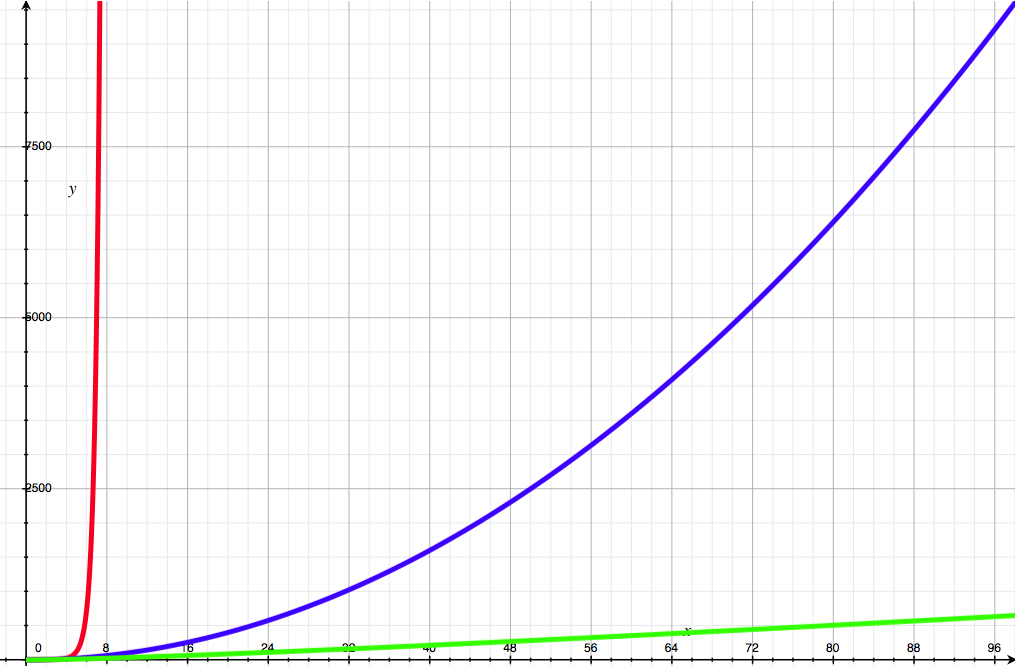
\includegraphics[width=0.7\textwidth]{./include/exs.png}
        \end{figure}
    \end{frame}


\section{Algoritme design}
    \begin{frame}[c]{Hvordan finder man på en algoritme}
        \begin{block}{Algoritme for algoritmer}
            \begin{enumerate}
                \item Beskriv problemet med egne ord. \pause
                \item Del problemet op i mindre dele. \pause
                \item Definer output \pause
                \item Definer input \pause
                \item Beskriv trin for at gå fra input til output
            \end{enumerate}
        \end{block}
    \end{frame}

    \begin{frame}[c]
        \centering \Huge{Så er det historie tid!}
    \end{frame}
\end{document}
